\chapter{The capillary fluctuation method revisited}
\label{ch:CFM}

%As discussed in detail in the previous chapter (\cref{sec:CFM}), the capillary fluctuation method is a technique that can be essentially divided in four ``steps''.
%\begin{enumerate}
%    \item \textbf{Defining an appropriate way to discriminate solid and liquid}. This is the very first step since the next goal will be that of ``locating'' in an atomistic system the dividing surface between the solid and the liquid phase.
%    
%    \item \textbf{Analysing the surface profile}. At this point we are able to distinguish atoms that belong to a solid--like environment and liquid--like ones; we can track down the position of the surface by collecting snapshots of its profile, $h$. The latter is in general a function of two variables, i.e.\ the coordinates (with respect to the chosen coordinate system) in the interface plane. At the end of the simulation, the profile function $h$ is Fourier transformed and an ensemble average is computed to obtain the so--called fluctuations spectrum.
%    
%    \item \textbf{Fitting the fluctuations spectrum}. Relations such as \cref{eqn:amplitudes,eqn:amplitudes_xy} give the explicit link between capillary fluctuations and surface stiffness $\sigma$. Through the fit of these non--linear models for different surfaces, we are able to completely determine the $\sigma$ tensor.
%    
%    \item \textbf{Extracting the anisotropy coefficients}. Since we know the relation between interface free energy and the stiffness and we have an approximation of the anisotropy of $\gamma$, we can analytically determine $\sigma$ from \cref{eqn:cubic_harmonics} and fit this against the value of the stiffness calculated previously. In this way we will obtain the two anisotropy coefficients  (here $\epsilon$ and $\delta$) and completely map out the dependence of $\gamma$ from the interface orientation.
%\end{enumerate}

We will explain here our method derived from the original CFM and present the preliminary results obtained for the stiffness for a simple Lennard--Jones system.


\section{Our method\label{sec:method}}
In this section we explain in full detail the method we developed for our calculations of the stiffness for a Lennard--Jones system,  devoting more attention to substantial differences with the original method developed by Asta.

%\subsubsection{Solid or liquid}
\subsection{Solid or liquid}
The very first requirement for a computational method whose aim is to study phase transitions or coexistence between different phases is a way of distinguishing particles belonging to the phases involved\footnote{Here we restrict ourselves to the case of solid and liquid, but it is clear that this prerequisite is completely general.}.

In molecular simulations of this kind, it is widespread to make use of a more or less complicate function that depends on atomic coordinates and that can give a quantitative indication of the ``order'' of one atom's neighborhood: this class of functions are usually called \emph{order parameters}. Many of these functions have been developed in order to face different problems; probably, the most known order parameters are the \textit{Steinhardt--Nelson} functions of different orders: $Q_3$, $Q_4$ and $Q_6$~\cite{Steinhardt1983}.

A common feature of all these order parameters is that they are some sort of average computed considering the coordinates of all the atoms and it should be intuitive that no function of this type is able to distinguish, for example, all the crystalline phases of a given system if they have different symmetry. In other words, a certain choice of an order parameter might be more suitable than another if one wants to study the environment of an HCP crystal rather than an FCC one.
Since all our systems (Lennard--Jones and real metal alloys) show at least one FCC crystalline phase, we chose the order parameter adopted also by Angioletti--Uberti~\cite{Angioletti-Uberti2010} and BCheng~\cite{Cheng2015} in their metadynamics calculations of interface free energy. This order parameter (henceforth called \fcc, $\Phi$) is defined as
\begin{equation}
\label{eqn:fccubic}
    \Phi(\bm{x}_i)=\frac{\sum_{j\neq i} C_r(\lvert \bm{x}_j-\bm{x}_i\rvert)\, C_{\alpha}(\bm{x}_j-\bm{x}_i) }{\sum_{j\neq i} C_r(\lvert \bm{x}_j-\bm{x}_i\rvert)}.
\end{equation}
The \fcc order parameter is a weighted average running over all pairs of atoms of an angular term ($C_{\alpha}$) and a ``weight'' which is a radial cutoff function ($C_r$) that ensures that $\Phi$ is a continuous function of all its arguments. The angular part can be specified using a set of Euler angles (by means of a Euler rotation matrix $\bm{R}$) and can be written as
\begin{equation}
\label{eqn:c_alpha}
C^{(\varphi,\psi,\theta)}_{\alpha} (\bm{r}_{ij})= C_{\alpha}(\bm{R}^{(\varphi,\psi,\theta)}\cdot \bm{r}_{ij}).
\end{equation}
Advantages of \fcc order parameter over the mentioned Steinhardt's $Q$ functions are, mainly: the angular part $C_{\alpha}$ has well--defined peaks for the FCC environment; it is not rotationally invariant and thus it is be able to recognize crystal orientations consistent with the imposed periodic boundary conditions; it is relatively cheap to compute. It is be possible to construct a different form of $C_{\alpha}$ if one wanted to deal with a different crystal structure,
and one simply has to rotate the function through the Euler matrix $\bm{R}$ in order to specify a different crystallographic orientation of the surface. The possibility of having an orientation--dependent order parameter is an essential ingredient of our method.

The ``final'' $\Phi$ actually used in our simulations is subject to few other mathematical manipulations mainly aimed to obtain that the perfect FCC lattice corresponds to $\Phi=1$, while the average value for atoms in bulk liquid is zero\footnote{This is ensured by applying a linear scaling of the kind%
\begin{equation*}
    \Phi(i)= \frac{\Phi^0(i)-\Phi^0_l}{\Phi^0_s-\Phi^0_l},
\end{equation*}
where $s$ and $l$ indicate the average of $\Phi$ on a bulk solid and liquid system respectively, and $\Phi^0$ is the unscaled order parameter defined above.
}. Lastly, since the distributions of such order parameter for a bulk solid system and a bulk liquid have a minimal amount of overlap (see \cref{fig:op-dist}), a non--linear switching function is applied to $\Phi$ in order to have a tunable and smooth variation from solid--like region to liquid--like\footnote{\label{ft:sf}In this case, the non--linear switching function applied has the form%
\begin{equation*}
    s(r)=\left[1+(2^{a/b}-1)\left( \frac{r-d_0}{r_0}\right)^a\right]^{-b/a},
\end{equation*}
where $r_0$ and $d_0$ are tunable parameters. For $r\le d_0\; s(r)=1$, while for $r>d_0$ the function decays smoothly to 0. 
}.
\begin{figure}[bt]
    \centering
    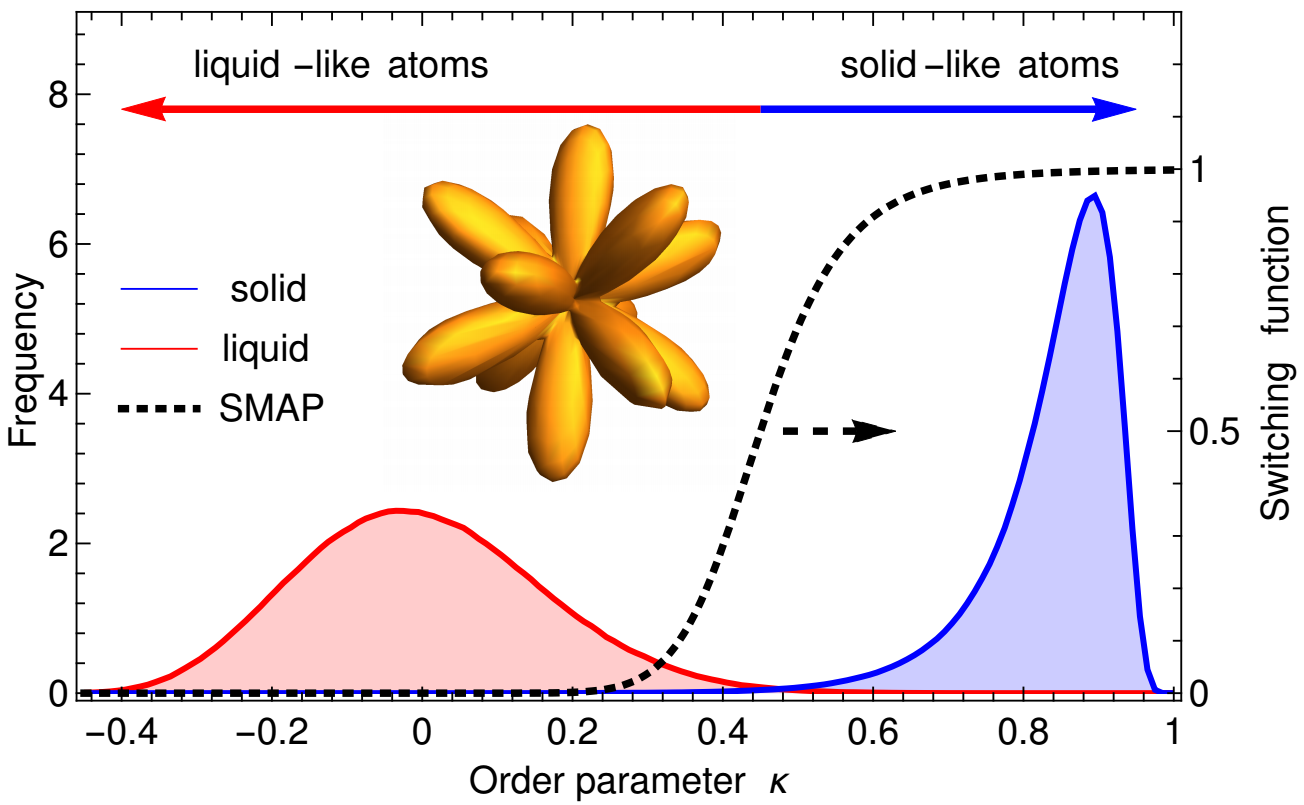
\includegraphics[width=.75\textwidth]{orderp-distribution}
    \caption{The distributions of the \fcc order parameter for a bulk FCC crystal oriented with $\langle 100\rangle$ directions parallel to the axes of the simulation cell. The distributions are computed at the equilibrium melting temperature. The dashed line is a plot of the switching function applied~~\cite{Cheng2015}.}
    \label{fig:op-dist}
\end{figure}




%\subsubsection{Looking for the dividing surface}
\subsection{Looking for the dividing surface}
In the work of Asta et al.\ they obtained the profile function of the dividing surface in the following way: they computed an FCC order parameter defined as $\phi=(1/12) \sum_i \lvert \bm{r}_i-\bm{r}_{fcc}\rvert^2$, where $\bm{r}_{fcc}$ is the distance between the central atom $i$ and its first 12 neighbours in the given orientation. Then, the $x$ direction in the simulation cell, parallel to the interface, is divided into slices and $\phi$ averaged over the slice is computed as a function of the $y$ direction (along the normal of the interface). As the solid--liquid interface is crossed, the value of $
\phi$ changes abruptly and the interface can be accurately located. By collecting snapshots of this function during all the simulation, one ends up with the time--varying profile function $h(y,t)$, where both the space and time coordinates are discretized.

The discrete nature of the profile function stems directly from the fact that the order parameter is a discrete quantity, since it assigns a numerical value to each atom. In turn, it means that the representation of the surface built in this way is highly sensitive on the $x$--width of the slices over which $\phi$ is averaged (i.e.\ the bin size). %Thus, this dividing surface will keep the atomistic

In our approach, we followed the idea proposed by Willard and Chandler~\cite{WilChaJCP2010}. To identify the liquid--vapour interface in water systems such that the resulting surface is to all effects a continuous function, they built a coarse--grained density field by computing the convolution of the instantaneous density field with a chosen kernel function. In this case, the kernel functions are taken to be normalized Gaussians, which depend on one parameter ($\xi$, the Gaussian width). So, in mathematical terms
\begin{equation}
\label{eqn:density-field}
    \begin{cases}
        \rho(\bm{r},t)=\sum_i \delta(\bm{r}-\bm{r}_i(t)) \\
        \kappa(\bm{r};\,\xi)= (2\pi\xi^2)^{-d/2} \exp{(-r^2/2\xi^2)}
    \end{cases}
    \xRightarrow{\text{convolution}}\quad
    \overline{\rho}(\bm{r},t)=\sum_i \kappa( |\bm{r}-\bm{r}_i(t)| );\,\xi)
\end{equation}
Here $r$ is the magnitude of the distance vector $\bm{r}$ and $\xi$ is the coarse--graining length; $d$ stands for the dimensionality of the system. As we will discuss in \cref{sec:results}, the importance of $\xi$ is that it controls the coarse nature of the continuous field obtained and it has to be chosen according to physical conditions under consideration.

From this idea for a simple density field to an \textit{order parameter density field}, the step is really short: it suffices modifying the instantaneous atomic ``density'' as follows
\begin{equation}
\label{eqn:op-field1}
    \rho(\bm{r},t) \leadsto \rho_{\phi}(\bm{r},t)=\sum_i \phi_i \delta(\bm{r}-\bm{r}_i(t)),
\end{equation}
and the coarse--grained field needs to be properly normalized
\begin{equation}
\label{eqn:op-field2}
    \overline{\rho}_{\phi}(\bm{r},t)= \frac{\sum_i \phi_i \kappa(\lvert \bm{r}-\bm{r}_i(t));\,\xi)}{\sum_i \kappa(\lvert \bm{r}-\bm{r}_i(t));\,\xi)}.
\end{equation}
Once $\xi$ is set, the dividing surface is defined to be the $(d-1)$--dimensional manifold $\bm{r}=\bm{s}$ for which
\begin{equation}
\label{eqn:field-equation}
     \overline{\rho}_{\phi}(\bm{s},t)=\mathpzc{C},
\end{equation}
where $\mathpzc{C}$ is some constant value. In other words, the instantaneous interface between solid and liquid is the locus of points in space where the order parameter density field assumes the value of $\mathpzc{C}$ (sometimes called \textit{isovalue}). It is clear that the choice of this constant is arbitrary, but it should rely on some meaningful physical consideration. Since the coarse--grained field changes with time as molecular configurations change, the surface is a two--dimensional function which depends on time only through atomic coordinates: $\bm{s}(t)=\bm{s}(\{\bm{r}_i(t)\})$.

For a given molecular configuration $\{\bm{r}_i\}$ at time $t$, \cref{eqn:field-equation} can be solved quickly with a variety of numerical algorithms, for example through interpolation on a spatial grid. If this equation is recast in the form $ \overline{\rho}_{\phi}(\bm{r},t)-\mathpzc{C}=0$, one among all the known root--finding algorithms can be exploited to solve it. We adopted the method due to Brent and Dekker\footnote{See {\ttfamily\url{https://en.wikipedia.org/wiki/Brent\%27s_method}}}, which has the reliability of the bisection method, but it is faster in convergence. 

Once an entire simulation for a specific interface is analysed, the interface profile function is Fourier transformed to obtain its fluctuation spectrum. Practical details of the simulations will be given in the next section; here it is sufficient to note that we employed the 2D geometry so that we needed only two independent surfaces to get the full anisotropy through the stiffness tensor. To get fluctuations amplitudes that appears in \cref{eqn:amplitudes_xy}, $h(\bm{x})$, where $\bm{x}$ is the vector with components $(x,y)$, is Fourier transformed according to
\begin{equation}
\label{eqn:FT}
    h(\bm{x},t)=\sum_{\bm{k}} A(\bm{k},t) \exp{(i\bm{k}\cdot\bm{x})}, 
\end{equation}
and $\bm{k}$ is the wave vector which takes the form $2\pi(j_x/L_x,\,j_y/L_y)$, with $j_x,\,j_y$ being non zero indexes and $L_x,\,L_y$ the size of the simulation cell in the interface plane.

The last step is to compute the ensemble (time) average of the fluctuation spectrum\footnote{Again, practical details on how this average has been calculate will be given when discussing results. Here we just note that, since time is discretized by definition in a MD simulation, we only have snapshots of the fluctuation spectrum and the time interval between two of these is a multiple of the timestep used in the MD simulation. Since an observable in consecutive snapshots may show a correlated behaviour, we exploited a way of computing the average in order to estimate correctly also the error on this average.}, where with ``spectrum'' we refer to the square moduli of the complex Fourier amplitudes. %:$|A(\bm{k},t)|^2 \leadsto \langle |A(\bm{k})|^2 \rangle$.

%One last detail is necessary to discuss: how to fix the constant value $\mathpzc{C}$ in order to solve \cref{eqn:field-equation}. In the original paper where this method was introduced, the authors were using the method to provide useful and instructive pictures of liquid--vapour and liquid--protein interfaces, particularly with water. For the case of the liquid--vapour dividing surface, they fixed the constant to one--half the density of liquid water in their system. %As already said, this choice contains some degree of arbitrariness, but it is still reasonable, since it is well--known that
%
%%In our case, a physically reasonable value for the constant would be the one that could clearly discriminate between a particle in a solid--like environment from one in the liquid--one. Unfortunately, as one can see from \cref{fig:op-dist}, there in no such sharp value. So, we firstly chose as $\mathpzc{C}$ the average value of the order parameter between an all solid system and an all liquid one, namely: $(\Phi_s+\Phi_l)/2$. However, we realized that such value was susceptible of appreciable changes if the interface was moving considerably due to fluctuations (larger in smaller cells) or if we changed the coarse--graining length $\xi$. Hence, we had the idea of transforming again the order parameter function by applying a second switching function: this function (see \cref{ft:sf}) was tuned so that the resulting order parameter had a really sharp change when traversing the diving surface; in this way, liquid atoms had a value of $\Phi$ very close to 0 and solid ones almost equal to 1. We could then fix the value of the constant to 0.5\footnote{Another small, but important detail hides in here: when computing the field as in \cref{eqn:op-field2}, the distance $|\bm{r}-\bm{r}_i|$ refers to a certain coordinate system with a fixed origin. It should be evident that changing the origin will influence the final result for $\rho_{\phi}$. So, in all our analysis, we fixed the origin by computing a weighted average position based on the values of the order parameter. Coordinates of the origin are defined according to
%\begin{equation*}
%    x_\alpha = \frac{1}{2\pi} \arctan \left[ \frac{ \sum_i w_i \Phi_i \sin\left( 2\pi x_{i,\alpha} \right) }{ \sum_i w_i \Phi_i \cos\left( 2\pi x_{i,\alpha} \right) } \right],
%\end{equation*}
%where $w_i$ are weights, $\Phi_i$ are the values of the order parameter and $x_{i,\alpha}$ the scaled Cartesian components of the position of the atoms. 
%All the analysis were run within the framework of the software \textsc{plumed}, with which is rather easy to compute such a quantity.}.



%\subsubsection{Fitting capillary fluctuations spectrum}
\subsection{Fitting capillary fluctuations spectrum}
To obtain the values of the stiffness tensor $\sigma$, the only thing left is fitting the averaged fluctuation spectrum with respect to $k$--vector, following the prescription of \cref{eqn:amplitudes_xy}: $T_m$ is known and the cross sectional area $S$ is simply the product $L_x\times L_y$. The only substantial difference here is a multiplicative term added to the fitting model, which changes into
\begin{equation}
\label{eqn:fit-model}
    \langle \lvert A(\bm{k}) \rvert^2 \rangle =\mathcal{P} \frac{\exp{(-k^2/2\xi^2)}}%
    %{\bm{k}\cdot\bm{\sigma}\cdot\bm{k}},
    %{\overline{k}^T\, \overline{\overline{\sigma}}\, \overline{k}},
    {k_x^2\sigma_{11} + k_y^2\sigma_{22} +2k_x k_y\sigma_{12}},
\end{equation}
where $\mathcal{P}=k_BT_m/S$ is the constant prefactor. %and $\bm{\sigma}$ is a second order tensor.
To explain why we added the exponential term, we recall that our representation of the surface is the result of a convolution of a Gaussian function with the order parameter density field. It is known that the Fourier transform of a convolution is the pointwise product of Fourier transforms and the Fourier transform of a Gaussian is again a Gaussian with a different width: this is the reason behind our modification of the fitting model.

% Results
\section{Preliminary results\label{sec:results}}
In this section the preliminary results for the stiffness of the simple Lennard--Jones system are presented. The models are to be considered as ``benchmark'' systems on which we tested our modified framework based on the CFM and with which results obtained in previous literature work are compared. All the simulations were run using the molecular dynamics simulator \textsc{lammps}~\cite{PlimptonLAMMPS1995} together with the software package \textsc{plumed}~\cite{Tribello2014}, used for all the analysis.

\subsection{The models}
As already explained, the CFM framework adopted allowed us to run only two independent simulations with different interface orientation. Specifically, (100) and (110) interface of an FCC crystal were chosen.

With the aim of verifying our revisited approach, we firstly studied capillary fluctuations in simple Lennard--Jones systems, leaving to future work the study of real alloy systems of concrete interest in additive manufacturing processes.

The potential used was a truncated Lennard--Jones potential~\cite{Cheng2015}:
\begin{equation}
    \label{eqn:LJ}
    V(r)=
    \begin{cases}
        4\epsilon\left[ \left(\frac{\sigma}{r}\right)^{12} - \left( \frac{\sigma}{r}\right)^6 \right] + C_1 & r\le 2.3\sigma \\
        C_2 \left(\frac{\sigma}{r}\right)^{12}+ C_3 \left(\frac{\sigma}{r}\right)^6 + C_4 \left(\frac{\sigma}{r}\right)^2 + C_5 & 2.3\sigma < r < 2.5\sigma \\
        0 & r\ge 2.5\sigma
    \end{cases}
\end{equation}
where $C_1=0.016132\epsilon$, $C_2=3136.6\epsilon$, $C_3=-68.069\epsilon$, $C_4=-0.083312\epsilon$ and $C_5=0.74689\epsilon$. The timestep was set equal to 0.004 time units in the Lennard--Jones scheme. The direction parallel to the interface normal was aligned with the $z$ axis and throughout all the simulations the $NP_zT$ ensemble was employed, with the Nose--Hoover thermostat and barostat to control pressure and temperature of the system.

The simulations for both the interfaces studied were run at the equilibrium melting temperature of 0.618 (in LJ units) and the initial crystalline systems were prepared considering the equilibrium lattice parameter at that temperature.

Models of both solid--liquid interfaces studied were generated as follows: once the interface of interest had been fixed, a perfect crystalline FCC unit cell was prepared with a lattice parameter consistent with the chosen temperature ($T_m$). The $z$ axis of the coordinate system was always aligned with the direction indicating the interface normal. Then, the unit cell has been replicated in the $xy$ plane and along $z$, always with a larger number of replicas in the $z$ direction, to ensure that solid and liquid regions were not too thin and statistical fluctuations too large.

First step of the simulations was actually generating the solid--liquid interface. To this end, a central slab of atoms has been held fixed: the size of this region depended on the length of the supercell in the $z$ direction (between $L_z/3$ and $2L_z/3$). A number of simulation steps ($\approx \num{25e3}$) were run in $NPT$ ensemble with the temperature fixed well above $T_m$, leading to complete melting of the two side regions of the supercell. Afterwards, the same number of steps were run with the target temperature of the thermostat being again fixed at $T_m$ and then a number of equilibration steps was carried out, letting all the atoms follow the unconstrained dynamics. With the protocol described, after approximately \num{1e5} MD steps, we obtained the equilibrated systems at the melting temperature with coexistence of solid and liquid regions. It is worth noting that no adjustment of the density was necessary when the liquid parts were generated, because the pressure was kept constant by the barostat and the volume was always free to fluctuate.



\subsection{(100) interface}
Following the recipe described above, to study (100) interface a supercell of $20\times 20 \times 50$ unit cells (in $x$, $y$ and $z$ direction respectively) was generated. The total number of atoms is \num{80000}. Since for an FCC crystal directions in direct space $[hkl]$ is perpendicular to the surface with the same Miller indexes\footnote{This statement is in general true for Bravais lattices with equal length basis vectors.}, the crystallographic axes were aligned along the standard Cartesian coordinate system.

\subsubsection{Grid spacing and bandwidth}
As the (100) model was the first to be studied, we ran preliminary tests changing the two tunable parameters when computing the order parameter field of \cref{eqn:op-field2}: the coarse--graining length $\xi$ and the spacing of the grid on which all the distances appearing in \cref{eqn:op-field2} were computed\footnote{In \cref{eqn:op-field2} the symbol $\bm{r}$ denotes an arbitrary position with respect to a chosen coordinate system. It is clear that, when computing the distance term in that expression, only a finite set of points in space can be ``sampled'': these points are those of a regular 3D grid, built considering the simulation box sizes and the spacing between two consecutive points in each direction.}.

For the grid spacing, we analysed the same trajectory of \num{1e6} steps (not counting the steps carried out for preparing the model, as described above) with the following different grid spacings: \numlist{0.25;0.5;1.0} (in LJ distance units). We noticed that only \num{1.0} gave an appreciable difference in the Fourier spectrum. This parameter controls the total number of grid points (and in turn the number of $k$ points, but not the smallest wave vector possible, which depends only on the simulation cell size), so a smaller value would mean having just more points for which to compute the distances with all the atoms; a value chosen within a reasonable range\footnote{``Big'' is far from specific: we can say that big would mean choosing a value much larger than the average distance between atoms; this choice would lead to a very coarse grid poorly sampling the simulation box.} does not affect much the result (i.e.\ the Fourier spectrum). For this reason, all the analysis were carried out with a grid spacing of \num{0.5}, a value that even for large simulation cells did not result in too expensive calculations.

The coarse--graining length (or bandwidth) $\xi$ deserves more attention, because this parameter also enters the model used afterwards to fit the Fourier spectrum and obtain the stiffness tensor.
We recall that the original model used for the fits has the form $A(k) \propto 1/k^2$, while our model has a multiplicative Gaussian term in addition: $A(k) \propto \exp{(-k^2/2\sigma_k^2)}/k^2$. As we built our order parameter density field by means of a convolution, Fourier transforming a Gaussian gives another Gaussian in $k$ space with the only difference in the bandwidth. Specifically, it holds the relation $\sigma_k = 1/\sigma$. Thus, we expect that a change in the $\xi$ used to build the coarse--grain field will influence the region of $k$ space over which the Gaussian smoothening shows its effect; in particular, the larger $\xi$, the narrower this region will be. As \cref{fig:bandwidths} shows, this is exactly what we obtained.
\begin{figure}[tb]
    \centering
    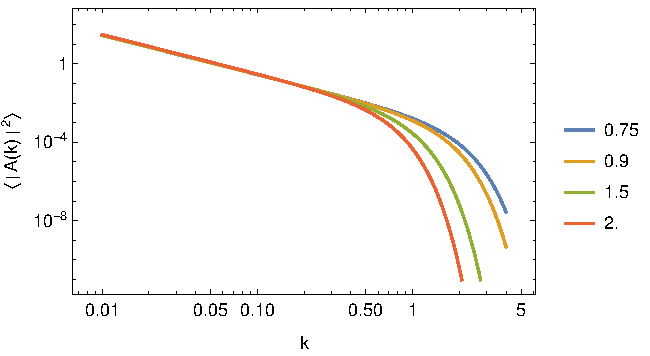
\includegraphics[width=.7\textwidth]{bandwidthComparison}
    \caption{Plots of the fitted Fourier spectrum with different values of $\xi$ used to build the coarse--grained field. Here $k$ stands for $k_x$.}
    \label{fig:bandwidths}
\end{figure}


\subsubsection{Computing the average Fourier spectrum}
As explained in \cref{sec:method}, the quantity subject to the fit as a function of $\bm{k}$ vectors is the average Fourier spectrum, $\langle |A(k_x,k_y)|^2 \rangle$. The easiest approach to compute this quantity, assuming valid the ergodicity postulate, would be to calculate for each $\bm{k}$ vector the time average of the corresponding Fourier amplitude (the square modulus of it). With this average it is also straightforward to compute the standard error of the mean.

The problem arises when dealing with time correlated data. Since we are studying fluctuations in Fourier spectrum, $\langle |A(\bm{k},t)|^2 \rangle$ is a clear example of data correlated in time. There are many ways to compute the correct error estimate of data of this kind. The main one consists of computing the \textit{time auto--correlation function}; the problem is that computing time correlation functions is usually expensive and requires a very frequent sampling (on the time scale) of the data. Another way of estimating statistical errors is studying the behaviour of so--called block averages~\cite{FrenkelSmitMD}.

What we did is a sort of combination of these two methods: since computing the time correlation function for every $\bm{k}$ point would have been too expensive, we considered only those $\bm{k}$ vectors with a zero component, namely $(2\pi j_x/L_x,0)$ and $(0,2\pi j_y/L_y)$. We then calculated the quantity called \textit{auto--correlation time}, $\tau$, which gives an estimate of how long one would have to ``wait'' between two consecutive samples of the measured observable to collect uncorrelated measures of it. Then, we used this information to compute the proper average and corrected error following the ``block average'' algorithm.

The idea of the block average is the following~\cite{Flyvbjerg1989}: let $A_1,A_2,\dots,A_L$ be $L$ consecutive samples of the quantity we want to calculate the average and its error. We now group our data in the following way
\begin{equation}
    A'_i= (A_{2i-1}+A_{2i})/2
\end{equation}
with $L'=0.5 L$. Clearly, the average of this ``new'' set of data is unchanged. The variance of this new set is given by
\begin{equation}
    \sigma^2(A')=\langle A'^2 \rangle - \langle A'\rangle^2=\frac{1}{L'}\sum_{i=1}^{L'} A'^2_i-\bar{A}'^2_i.
\end{equation}
If we perform again this blocking operation (taking, instead of pairs of data, group of three) and if we have a simulation long enough, the averages $A'_i$ will become completely uncorrelated. This means that the following relation would hold
\begin{equation}
    \frac{\sigma^2(A')}{L'-1}\approx \text{constant}.
\end{equation}
In a similar way, we can also determine the statistical error of $\sigma^2(A')$, which would give an estimate of the variance in our ensemble average
\begin{equation}
\label{eqn:error-blocked}
    \sigma^2(A) \approx \frac{\sigma^2(A')}{L'-1} \pm \sqrt{\frac{2\sigma^4(A')}{(L'-1)^3}}.
\end{equation}
In our case, we have also an estimate of the auto--correlation time $\tau$, so we can avoid the full block average calculation and compute the error given by \cref{eqn:error-blocked} with a block size $L'$ corresponding to a time interval of $\sim 2\tau$. In this way the final ensemble average will have an error estimate corrected taking into account time correlation.

\subsubsection{Stiffness tensor for (100)}
Having explained all the technical details, we present in this section the results for the stiffness tensor obtained in our simulations. According to the analysis explained in the previous section, the average of the Fourier spectrum and its error estimates were computed considering blocks of 72 frames.

Since (100) is a highly symmetric surface for the FCC system, it can be shown that the following relations hold for the stiffness tensor, $\sigma$: $\sigma_{11}=\sigma_{22}$ and $\sigma_{12}$ is zero. \Cref{tab:stiffness} summarizes the results obtained and compares them with the values of~\textcite{Becker2009:CFM2D}\footnote{In this work, the fitting model is a symmetry--consistent model, that is for the (100) only one value of the stiffness tensor was considered. The model is identical to the one used for one--dimensional interfaces.}.
\begin{table}[tb]
    \centering
    \caption{Stiffness values calculated by our method at \num{0.6185} reduced temperature for (100) interface. Units on stiffness are $(\epsilon/\sigma^2)$. The values obtained by Becker at the same temperature are also reported for comparison (95\% confidence level on the last digit).}
    \begin{tabular}{lcccc}
        \toprule
        \multirow{2}*{Interface  $(hkl)$} & \multicolumn{3}{c}{Present work} & Ref.~\cite{Becker2009:CFM2D}\\
        \cmidrule(r){2-4}
        & $\sigma_{11}$ & $\sigma_{22}$ & $\sigma_{12}$ & $\sigma$\\
        \midrule
        $(100)$ & $0.2897\pm \num{8.0e-4}$ & $0.2871\pm \num{7.0e-4}$ &\num{4.6e-18} & \num{0.2866} \\
        %$(110)$ & $\num{0.379}\pm \num{1.0e-3}$  & $\num{0.316}\pm \num{1.0e-3} $ & \num{1.13e-19} & \num{0.431} & \num{0.305} \\
         \bottomrule
    \end{tabular}
    \label{tab:stiffness}
\end{table}




%\subsection{(110) interface}
%The model used to study (110) interface was prepared in the same way as the one for the (100); the only differences are the number of unit cells for each direction of the supercell ($20\times 20\times 30$) and the directions along which the Cartesian axes where aligned: $x$ axis is along $[\bar{1}10]$, $y$ along $[001]$ and $z$ along $[110]$, that is the normal to the interface $(110)$. Incidentally, this is the same configuration adopted by~\textcite{Becker2009:CFM2D}. The results obtained for the stiffness tensor are reported in \cref{tab:stiffness}. In this case, average of the Fourier spectrum was computed with block of 6 frames.